%\section{Analysis of the adjustment factor}
%Figure~\ref{fig:factors} shows the scatter of $\eta_{inc}$ and $\eta_{ads}$ for the studied cases. The corresponding numeric values are reported in Table~\ref{tab:optimizedfactors}. The data points obtained using KAUST for each inception model are overall lower than those obtained by Caltech because of the higher PAH production rates predicted using KAUST, which can be inferred from the higher maximum possible $f_v$ in Figure~\ref{fig:max_sootfv_chem}.

%\begin{figure}[H]
%	\centering
%	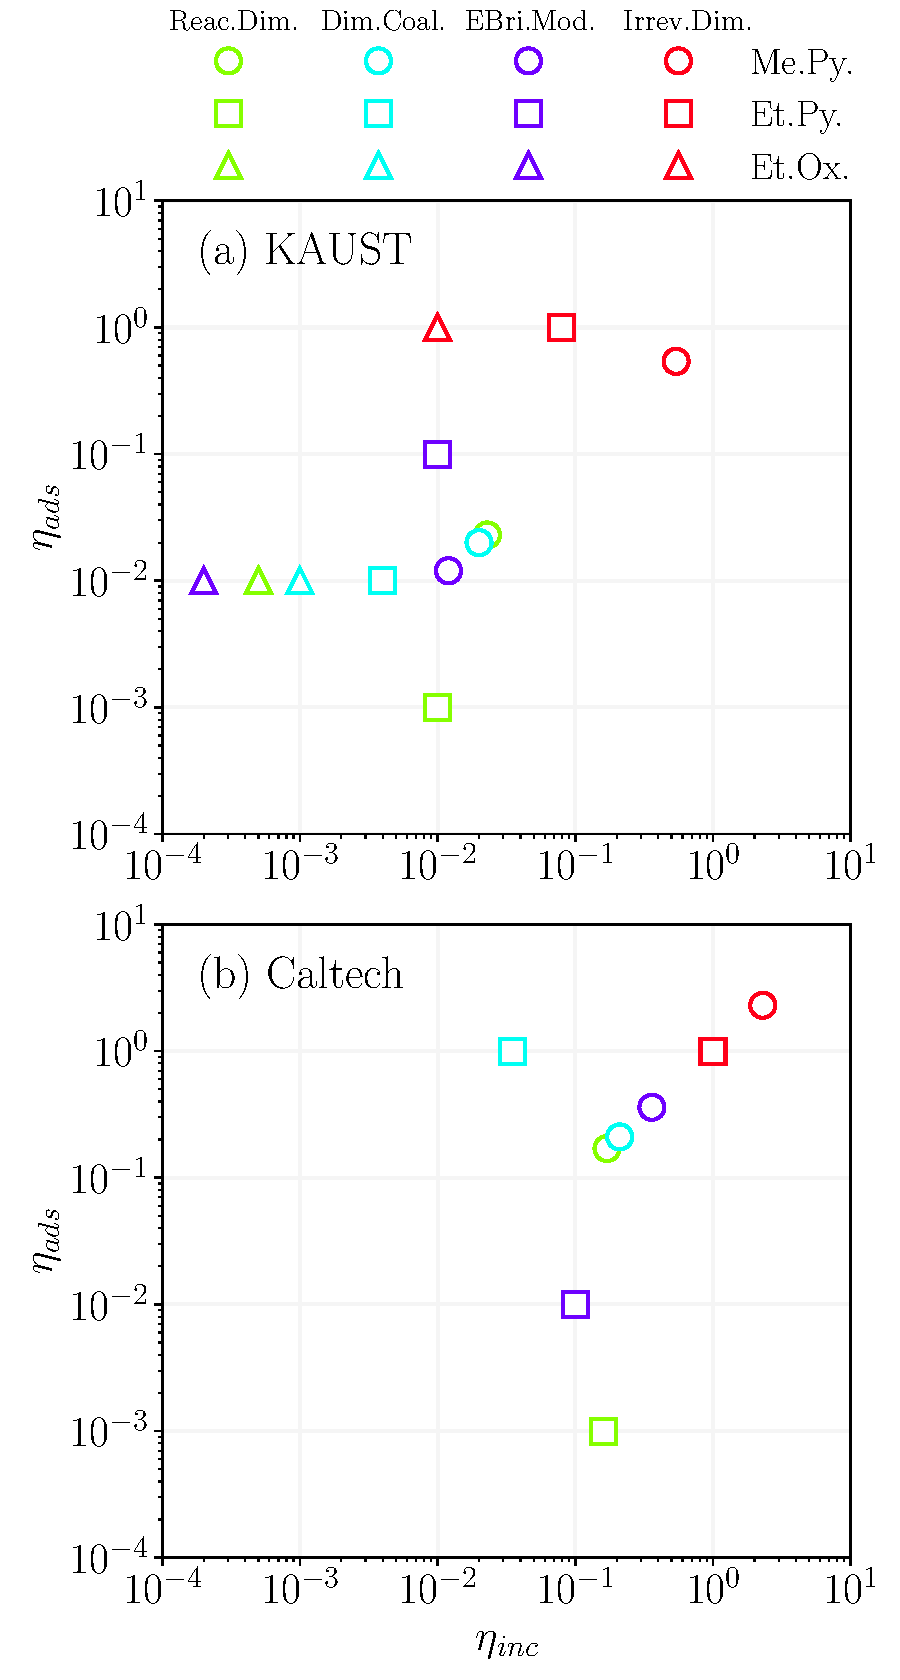
\includegraphics[width=0.33\textwidth]{Figures/Results/factors/factors.pdf}
%	\caption{The scatters of $\eta_{inc}$ and $\eta_{ads}$ used to minimize the  prediction error with measurements in the methane pyrolysis in a shock tube (labeled as ``Me.Py."), the ethylene pyrolysis in a flow reactor(labeled as ``Et.Py."), and the ethylene oxidation in a perfectly stirred reactor (labeled as ``Et.Ox.") using the KAUST (a) and Caltech (b) mechanisms.}
%	\label{fig:factors} 
%\end{figure}